\documentclass{extbook}[14pt]
\usepackage{multicol, enumerate, enumitem, hyperref, color, soul, setspace, parskip, fancyhdr, amssymb, amsthm, amsmath, latexsym, units, mathtools}
\everymath{\displaystyle}
\usepackage[headsep=0.5cm,headheight=0cm, left=1 in,right= 1 in,top= 1 in,bottom= 1 in]{geometry}
\usepackage{dashrule}  % Package to use the command below to create lines between items
\newcommand{\litem}[1]{\item #1

\rule{\textwidth}{0.4pt}}
\pagestyle{fancy}
\lhead{}
\chead{Answer Key for Progress Quiz 8 Version C}
\rhead{}
\lfoot{5493-4176}
\cfoot{}
\rfoot{Summer C 2021}
\begin{document}
\textbf{This key should allow you to understand why you choose the option you did (beyond just getting a question right or wrong). \href{https://xronos.clas.ufl.edu/mac1105spring2020/courseDescriptionAndMisc/Exams/LearningFromResults}{More instructions on how to use this key can be found here}.}

\textbf{If you have a suggestion to make the keys better, \href{https://forms.gle/CZkbZmPbC9XALEE88}{please fill out the short survey here}.}

\textit{Note: This key is auto-generated and may contain issues and/or errors. The keys are reviewed after each exam to ensure grading is done accurately. If there are issues (like duplicate options), they are noted in the offline gradebook. The keys are a work-in-progress to give students as many resources to improve as possible.}

\rule{\textwidth}{0.4pt}

\begin{enumerate}\litem{
Construct the lowest-degree polynomial given the zeros below. Then, choose the intervals that contain the coefficients of the polynomial in the form $ax^3+bx^2+cx+d$.
\[ \frac{-5}{2}, \frac{4}{3}, \text{ and } -1 \]The solution is \( 6x^{3} +13 x^{2} -13 x -20 \), which is option D.\begin{enumerate}[label=\Alph*.]
\item \( a \in [1, 10], b \in [13, 15], c \in [-15, -4], \text{ and } d \in [10, 26] \)

$6x^{3} +13 x^{2} -13 x + 20$, which corresponds to multiplying everything correctly except the constant term.
\item \( a \in [1, 10], b \in [-2, 5], c \in [-31, -24], \text{ and } d \in [-22, -12] \)

$6x^{3} -1 x^{2} -27 x -20$, which corresponds to multiplying out $(2x -5)(3x + 4)(x + 1)$.
\item \( a \in [1, 10], b \in [-14, -11], c \in [-15, -4], \text{ and } d \in [10, 26] \)

$6x^{3} -13 x^{2} -13 x + 20$, which corresponds to multiplying out $(2x -5)(3x + 4)(x -1)$.
\item \( a \in [1, 10], b \in [13, 15], c \in [-15, -4], \text{ and } d \in [-22, -12] \)

* $6x^{3} +13 x^{2} -13 x -20$, which is the correct option.
\item \( a \in [1, 10], b \in [-19, -15], c \in [-3, -2], \text{ and } d \in [10, 26] \)

$6x^{3} -17 x^{2} -3 x + 20$, which corresponds to multiplying out $(2x -5)(3x -4)(x + 1)$.
\end{enumerate}

\textbf{General Comment:} To construct the lowest-degree polynomial, you want to multiply out $(2x + 5)(3x -4)(x + 1)$
}
\litem{
Describe the end behavior of the polynomial below.
\[ f(x) = 2(x - 3)^{5}(x + 3)^{10}(x + 7)^{4}(x - 7)^{5} \]The solution is the graph below, which is option C.
    \begin{center}
        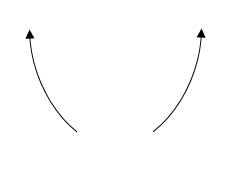
\includegraphics[width=0.3\textwidth]{../Figures/polyEndBehaviorCopyCC.png}
    \end{center}\begin{enumerate}[label=\Alph*.]
\begin{multicols}{2}
\item 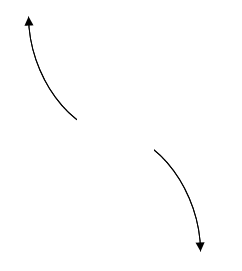
\includegraphics[width = 0.3\textwidth]{../Figures/polyEndBehaviorCopyAC.png}
\item 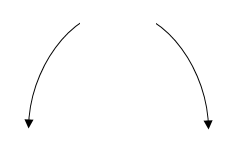
\includegraphics[width = 0.3\textwidth]{../Figures/polyEndBehaviorCopyBC.png}
\item 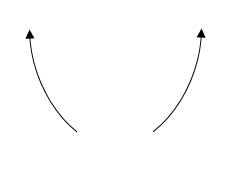
\includegraphics[width = 0.3\textwidth]{../Figures/polyEndBehaviorCopyCC.png}
\item 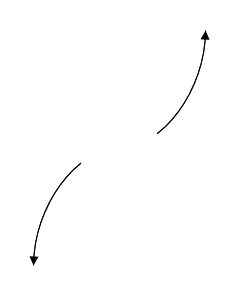
\includegraphics[width = 0.3\textwidth]{../Figures/polyEndBehaviorCopyDC.png}
\end{multicols}\item None of the above.\end{enumerate}
\textbf{General Comment:} Remember that end behavior is determined by the leading coefficient AND whether the \textbf{sum} of the multiplicities is positive or negative.
}
\litem{
Construct the lowest-degree polynomial given the zeros below. Then, choose the intervals that contain the coefficients of the polynomial in the form $x^3+bx^2+cx+d$.
\[ -3 - 5 i \text{ and } -4 \]The solution is \( x^{3} +10 x^{2} +58 x + 136 \), which is option C.\begin{enumerate}[label=\Alph*.]
\item \( b \in [-11, -8], c \in [57.4, 58.57], \text{ and } d \in [-141, -128] \)

$x^{3} -10 x^{2} +58 x -136$, which corresponds to multiplying out $(x-(-3 - 5 i))(x-(-3 + 5 i))(x -4)$.
\item \( b \in [1, 5], c \in [8.96, 9.07], \text{ and } d \in [16, 25] \)

$x^{3} + x^{2} +9 x + 20$, which corresponds to multiplying out $(x + 5)(x + 4)$.
\item \( b \in [9, 15], c \in [57.4, 58.57], \text{ and } d \in [136, 145] \)

* $x^{3} +10 x^{2} +58 x + 136$, which is the correct option.
\item \( b \in [1, 5], c \in [6.8, 8.11], \text{ and } d \in [12, 18] \)

$x^{3} + x^{2} +7 x + 12$, which corresponds to multiplying out $(x + 3)(x + 4)$.
\item \( \text{None of the above.} \)

This corresponds to making an unanticipated error or not understanding how to use nonreal complex numbers to create the lowest-degree polynomial. If you chose this and are not sure what you did wrong, please contact the coordinator for help.
\end{enumerate}

\textbf{General Comment:} Remember that the conjugate of $a+bi$ is $a-bi$. Since these zeros always come in pairs, we need to multiply out $(x-(-3 - 5 i))(x-(-3 + 5 i))(x-(-4))$.
}
\litem{
Describe the end behavior of the polynomial below.
\[ f(x) = -2(x - 8)^{4}(x + 8)^{5}(x + 4)^{2}(x - 4)^{2} \]The solution is the graph below, which is option A.
    \begin{center}
        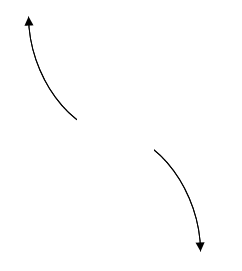
\includegraphics[width=0.3\textwidth]{../Figures/polyEndBehaviorAC.png}
    \end{center}\begin{enumerate}[label=\Alph*.]
\begin{multicols}{2}
\item 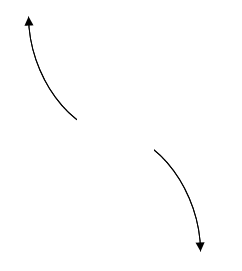
\includegraphics[width = 0.3\textwidth]{../Figures/polyEndBehaviorAC.png}
\item 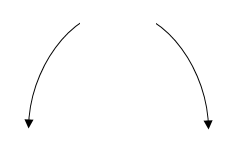
\includegraphics[width = 0.3\textwidth]{../Figures/polyEndBehaviorBC.png}
\item 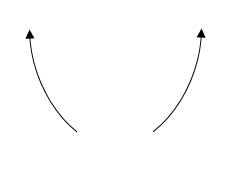
\includegraphics[width = 0.3\textwidth]{../Figures/polyEndBehaviorCC.png}
\item 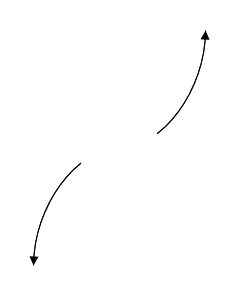
\includegraphics[width = 0.3\textwidth]{../Figures/polyEndBehaviorDC.png}
\end{multicols}\item None of the above.\end{enumerate}
\textbf{General Comment:} Remember that end behavior is determined by the leading coefficient AND whether the \textbf{sum} of the multiplicities is positive or negative.
}
\litem{
Which of the following equations \textit{could} be of the graph presented below?

\begin{center}
    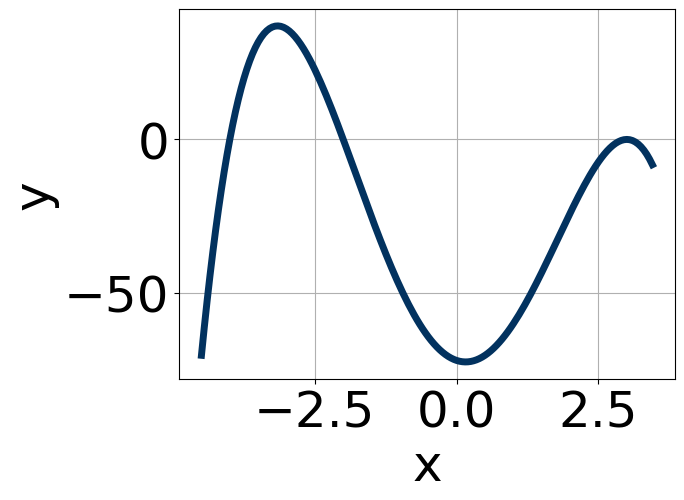
\includegraphics[width=0.5\textwidth]{../Figures/polyGraphToFunctionCopyC.png}
\end{center}


The solution is \( -14(x - 3)^{8} (x + 4)^{11} (x + 2)^{5} \), which is option E.\begin{enumerate}[label=\Alph*.]
\item \( -2(x - 3)^{6} (x + 4)^{10} (x + 2)^{5} \)

The factor $(x + 4)$ should have an odd power.
\item \( 6(x - 3)^{10} (x + 4)^{11} (x + 2)^{7} \)

This corresponds to the leading coefficient being the opposite value than it should be.
\item \( 19(x - 3)^{6} (x + 4)^{9} (x + 2)^{10} \)

The factor $(x + 2)$ should have an odd power and the leading coefficient should be the opposite sign.
\item \( -19(x - 3)^{9} (x + 4)^{6} (x + 2)^{11} \)

The factor $3$ should have an even power and the factor $-4$ should have an odd power.
\item \( -14(x - 3)^{8} (x + 4)^{11} (x + 2)^{5} \)

* This is the correct option.
\end{enumerate}

\textbf{General Comment:} General Comments: Draw the x-axis to determine which zeros are touching (and so have even multiplicity) or cross (and have odd multiplicity).
}
\litem{
Describe the zero behavior of the zero $x = 9$ of the polynomial below.
\[ f(x) = 2(x + 5)^{4}(x - 5)^{2}(x + 9)^{11}(x - 9)^{8} \]The solution is the graph below, which is option C.
    \begin{center}
        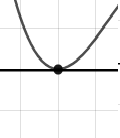
\includegraphics[width=0.3\textwidth]{../Figures/polyZeroBehaviorCC.png}
    \end{center}\begin{enumerate}[label=\Alph*.]
\begin{multicols}{2}
\item 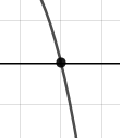
\includegraphics[width = 0.3\textwidth]{../Figures/polyZeroBehaviorAC.png}
\item 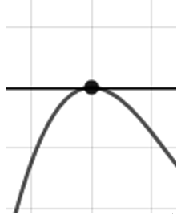
\includegraphics[width = 0.3\textwidth]{../Figures/polyZeroBehaviorBC.png}
\item 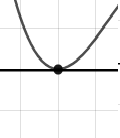
\includegraphics[width = 0.3\textwidth]{../Figures/polyZeroBehaviorCC.png}
\item 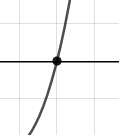
\includegraphics[width = 0.3\textwidth]{../Figures/polyZeroBehaviorDC.png}
\end{multicols}\item None of the above.\end{enumerate}
\textbf{General Comment:} You will need to sketch the entire graph, then zoom in on the zero the question asks about.
}
\litem{
Construct the lowest-degree polynomial given the zeros below. Then, choose the intervals that contain the coefficients of the polynomial in the form $x^3+bx^2+cx+d$.
\[ 5 + 3 i \text{ and } -2 \]The solution is \( x^{3} -8 x^{2} +14 x + 68 \), which is option D.\begin{enumerate}[label=\Alph*.]
\item \( b \in [-3, 4], c \in [-1, 3], \text{ and } d \in [-8, -3] \)

$x^{3} + x^{2} -x -6$, which corresponds to multiplying out $(x -3)(x + 2)$.
\item \( b \in [5, 14], c \in [7, 19], \text{ and } d \in [-75, -65] \)

$x^{3} +8 x^{2} +14 x -68$, which corresponds to multiplying out $(x-(5 + 3 i))(x-(5 - 3 i))(x -2)$.
\item \( b \in [-3, 4], c \in [-7, -2], \text{ and } d \in [-10, -8] \)

$x^{3} + x^{2} -3 x -10$, which corresponds to multiplying out $(x -5)(x + 2)$.
\item \( b \in [-12, -7], c \in [7, 19], \text{ and } d \in [67, 75] \)

* $x^{3} -8 x^{2} +14 x + 68$, which is the correct option.
\item \( \text{None of the above.} \)

This corresponds to making an unanticipated error or not understanding how to use nonreal complex numbers to create the lowest-degree polynomial. If you chose this and are not sure what you did wrong, please contact the coordinator for help.
\end{enumerate}

\textbf{General Comment:} Remember that the conjugate of $a+bi$ is $a-bi$. Since these zeros always come in pairs, we need to multiply out $(x-(5 + 3 i))(x-(5 - 3 i))(x-(-2))$.
}
\litem{
Construct the lowest-degree polynomial given the zeros below. Then, choose the intervals that contain the coefficients of the polynomial in the form $ax^3+bx^2+cx+d$.
\[ \frac{-2}{3}, \frac{7}{3}, \text{ and } 6 \]The solution is \( 9x^{3} -69 x^{2} +76 x + 84 \), which is option A.\begin{enumerate}[label=\Alph*.]
\item \( a \in [3, 10], b \in [-71, -67], c \in [69, 84], \text{ and } d \in [82, 94] \)

* $9x^{3} -69 x^{2} +76 x + 84$, which is the correct option.
\item \( a \in [3, 10], b \in [-71, -67], c \in [69, 84], \text{ and } d \in [-86, -79] \)

$9x^{3} -69 x^{2} +76 x -84$, which corresponds to multiplying everything correctly except the constant term.
\item \( a \in [3, 10], b \in [66, 74], c \in [69, 84], \text{ and } d \in [-86, -79] \)

$9x^{3} +69 x^{2} +76 x -84$, which corresponds to multiplying out $(3x -2)(3x + 7)(x + 6)$.
\item \( a \in [3, 10], b \in [-43, -34], c \in [-106, -100], \text{ and } d \in [82, 94] \)

$9x^{3} -39 x^{2} -104 x + 84$, which corresponds to multiplying out $(3x -2)(3x + 7)(x -6)$.
\item \( a \in [3, 10], b \in [-81, -79], c \in [175, 180], \text{ and } d \in [-86, -79] \)

$9x^{3} -81 x^{2} +176 x -84$, which corresponds to multiplying out $(3x -2)(3x -7)(x -6)$.
\end{enumerate}

\textbf{General Comment:} To construct the lowest-degree polynomial, you want to multiply out $(3x + 2)(3x -7)(x -6)$
}
\litem{
Which of the following equations \textit{could} be of the graph presented below?

\begin{center}
    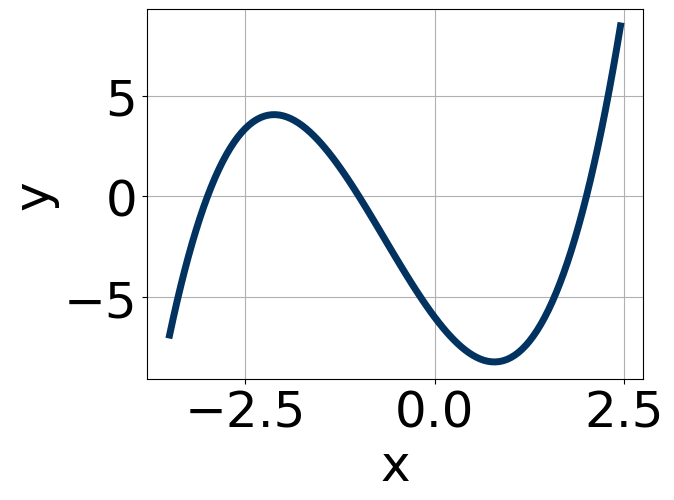
\includegraphics[width=0.5\textwidth]{../Figures/polyGraphToFunctionC.png}
\end{center}


The solution is \( 20(x - 2)^{7} (x + 3)^{5} (x + 1)^{9} \), which is option B.\begin{enumerate}[label=\Alph*.]
\item \( 12(x - 2)^{6} (x + 3)^{5} (x + 1)^{7} \)

The factor $2$ should have been an odd power.
\item \( 20(x - 2)^{7} (x + 3)^{5} (x + 1)^{9} \)

* This is the correct option.
\item \( -17(x - 2)^{4} (x + 3)^{7} (x + 1)^{5} \)

The factor $(x - 2)$ should have an odd power and the leading coefficient should be the opposite sign.
\item \( -14(x - 2)^{7} (x + 3)^{11} (x + 1)^{7} \)

This corresponds to the leading coefficient being the opposite value than it should be.
\item \( 9(x - 2)^{4} (x + 3)^{6} (x + 1)^{9} \)

The factors $2$ and $-3$ have have been odd power.
\end{enumerate}

\textbf{General Comment:} General Comments: Draw the x-axis to determine which zeros are touching (and so have even multiplicity) or cross (and have odd multiplicity).
}
\litem{
Describe the zero behavior of the zero $x = 4$ of the polynomial below.
\[ f(x) = 5(x - 4)^{9}(x + 4)^{10}(x - 7)^{9}(x + 7)^{10} \]The solution is the graph below, which is option A.
    \begin{center}
        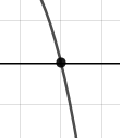
\includegraphics[width=0.3\textwidth]{../Figures/polyZeroBehaviorCopyAC.png}
    \end{center}\begin{enumerate}[label=\Alph*.]
\begin{multicols}{2}
\item 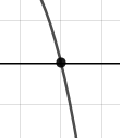
\includegraphics[width = 0.3\textwidth]{../Figures/polyZeroBehaviorCopyAC.png}
\item 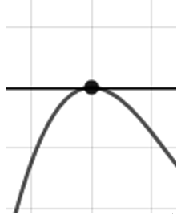
\includegraphics[width = 0.3\textwidth]{../Figures/polyZeroBehaviorCopyBC.png}
\item 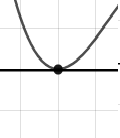
\includegraphics[width = 0.3\textwidth]{../Figures/polyZeroBehaviorCopyCC.png}
\item 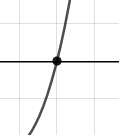
\includegraphics[width = 0.3\textwidth]{../Figures/polyZeroBehaviorCopyDC.png}
\end{multicols}\item None of the above.\end{enumerate}
\textbf{General Comment:} You will need to sketch the entire graph, then zoom in on the zero the question asks about.
}
\end{enumerate}

\end{document}